\documentclass[9pt]{extarticle}
\usepackage[letterpaper,margin=0.72in,top=0.62in,bottom=0.68in]{geometry}
\usepackage[T1]{fontenc}
\usepackage{lmodern}
\usepackage{microtype}
\usepackage{amsmath,amssymb}
\usepackage{booktabs,tabularx,array}
\usepackage{enumitem}
\usepackage{xcolor}
\usepackage{tikz}
\usetikzlibrary{arrows.meta,positioning,fit,shapes.geometric}
\usepackage{graphicx}
\usepackage{caption}
\usepackage{subcaption}
\usepackage{fancyhdr}
\usepackage[hidelinks]{hyperref}
\usepackage{titlesec}
\usepackage{url}
\usepackage{float}
\usepackage{placeins}

\definecolor{tagblue}{HTML}{164E63}
\definecolor{tagcyan}{HTML}{0891B2}
\definecolor{taglight}{HTML}{ECFEFF}
\definecolor{tagorange}{HTML}{C2410C}
\definecolor{taggray}{HTML}{475569}
\hypersetup{colorlinks=true,linkcolor=tagblue,citecolor=tagblue,urlcolor=tagcyan}

\pagestyle{fancy}
\fancyhf{}
\lhead{COOL AUTONOMY LAB --- TAG}
\rhead{Truong and Nguyen}
\cfoot{\thepage}
\setlength{\headheight}{13pt}
\setlength{\parindent}{0.16in}
\setlength{\parskip}{2pt}
\setlist[itemize]{leftmargin=1.35em,itemsep=2pt,topsep=2pt}
\setlist[enumerate]{leftmargin=1.5em,itemsep=2pt,topsep=2pt}
\titlespacing*{\section}{0pt}{7pt}{3pt}
\titlespacing*{\subsection}{0pt}{5pt}{2pt}
\titleformat{\section}{\large\bfseries\color{tagblue}}{\thesection.}{0.45em}{}
\titleformat{\subsection}{\normalsize\bfseries\color{taggray}}{\thesubsection}{0.4em}{}
\captionsetup{font=small,labelfont=bf,skip=3pt}
\setlength{\textfloatsep}{7pt plus 2pt minus 2pt}
\setlength{\intextsep}{6pt plus 2pt minus 2pt}
\setlength{\floatsep}{6pt plus 2pt minus 2pt}
\raggedbottom

\newcommand{\code}[1]{\texttt{#1}}
\newcommand{\callout}[2]{%
\begin{center}
\begin{tikzpicture}
\node[draw=tagcyan,fill=taglight,rounded corners=2pt,inner sep=6pt,text width=0.92\linewidth] {\textbf{#1} #2};
\end{tikzpicture}
\end{center}}

\begin{document}

\begin{center}
{\LARGE\bfseries\color{tagblue} TAG: Testbed for Autonomous Games \\[2pt] Labyrinth with a Top-Mounted Rotary Inverted Pendulum}\par
\vspace{5pt}
{\large Trung Bao Truong, Thanh Dat Nguyen}\par
{\small Control, Optimization, and Online Learning (COOL) for Autonomy Lab}\par
{\small Department of Aerospace Engineering and Engineering Mechanics}\par
{\small The University of Texas at Austin}\par
\end{center}

\begin{abstract}
TAG is a real labyrinth robot designed for reinforcement-learning experiments. Two servos tilt the maze, a camera tracks the marble, and a rotary inverted pendulum is mounted at the center of the board. The pendulum makes the task more challenging because its motion introduces reaction torque and vibration into the same structure that controls the marble. DreamerV3 serves as the high-level maze controller. It receives the maze image, board angles, marble position and measured velocity, future path points, and optional pendulum data. Its actions are converted into desired pitch and roll angles for the two maze servos. This paper explains how the learning algorithm is connected to the physical hardware, which neural-network components are used within DreamerV3, why its recurrent world model is currently preferred over a Transformer, and what was learned from the initial training run. We also developed an integrated NVIDIA Isaac Sim environment that models the labyrinth, marble, tilting board, and top-mounted rotary inverted pendulum within the same rigid-body simulation. This environment enables the maze controller to be trained and evaluated while pendulum motion disturbs the supporting board. Simulation accelerates experience collection and permits early policy exploration without motor heating, cooldown periods, mechanical wear, repeated manual resets, or risk to the physical platform. Because actuator delay, friction, contact, sensor noise, structural compliance, and vibration cannot be reproduced perfectly, simulated pretraining is followed by system identification and hardware fine-tuning.
\end{abstract}

\section{Introduction}
The goal of TAG is easy to describe: move a marble from the start of a maze to the end without falling into a hole. The real problem is much harder. The marble has momentum, the board has actuator delay, the camera is not perfect, and contact with a wall can change the motion quickly. In our platform, the Rotary Inverted Pendulum (RIP) is mounted directly on the maze. Its motor and rotating mass add vibration and reaction torque to the board.

CyberRunner showed that model-based reinforcement learning can learn a real labyrinth directly from camera experience~\cite{bi2023cyberrunner,cyberrepo2026}. TAG follows the same general idea, but our platform adds the top-mounted pendulum, a different servo system, a compact learned marble detector, stronger state checks, remote GPU training, and safety tools for long experiments. The goal is not to claim that TAG already performs better. The goal is to build a platform where we can study learning under disturbance and later test transfer to new maps.

\section{TAG System Overview}
At each control step, the camera sends an image to the robot computer. The state estimator finds the marble, estimates the board pose, and converts the result into maze coordinates. The observation is sent to the GPU server, where DreamerV3 chooses the next board-angle command. The two Hiwonder LX-16A servos then move to the requested pitch and roll positions. The new observation, reward, and action are stored in replay so the same physical experience can be used for many training updates.

\begin{figure}[H]
\centering
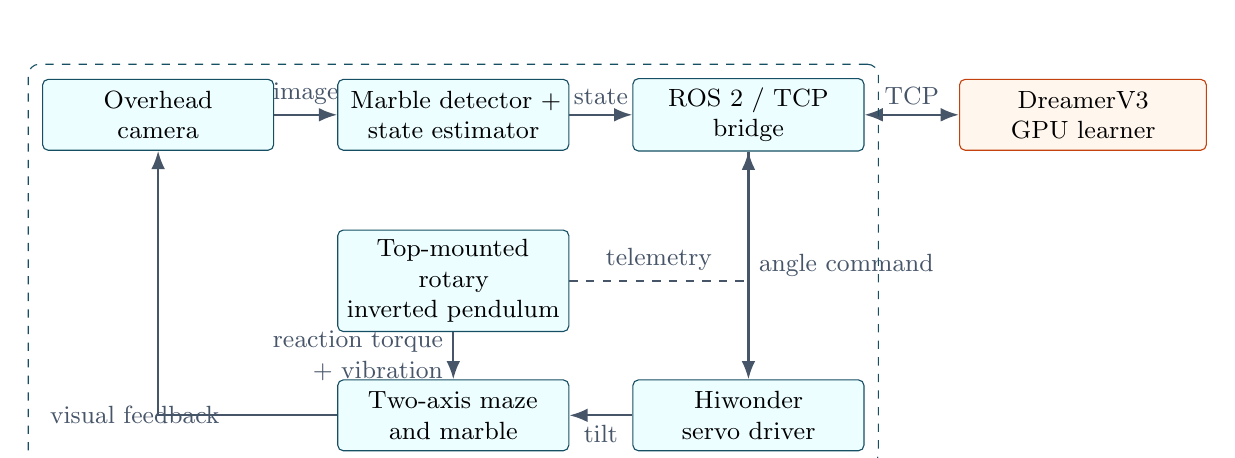
\begin{tikzpicture}[node distance=7mm and 8mm,>=Latex,font=\small]
\tikzset{box/.style={draw=tagblue,rounded corners=2pt,minimum height=9mm,align=center,fill=taglight,text width=27mm},
server/.style={draw=tagorange,rounded corners=2pt,minimum height=9mm,align=center,fill=orange!7,text width=29mm},
arr/.style={->,thick,color=taggray}}
\node[box] (cam) {Overhead\\camera};
\node[box,right=of cam] (est) {Marble detector +\\state estimator};
\node[box,right=of est] (bridge) {ROS 2 / TCP\\bridge};
\node[server,right=12mm of bridge] (agent) {DreamerV3\\GPU learner};
\node[box,below=10mm of est] (rip) {Top-mounted rotary\\inverted pendulum};
\node[box,below=6mm of rip] (board) {Two-axis maze\\and marble};
\node[box,right=of board] (servo) {Hiwonder\\servo driver};
\draw[arr] (cam)--node[above]{image}(est);
\draw[arr] (est)--node[above]{state}(bridge);
\draw[arr,<->] (bridge)--node[above]{TCP}(agent);
\draw[arr] (bridge)--node[right]{angle command}(servo);
\draw[arr] (servo)--node[below]{tilt}(board);
\draw[arr] (rip)--node[left,align=right]{reaction torque\\+ vibration}(board);
\draw[arr,dashed] (rip.east) -| node[pos=.25,above]{telemetry} (bridge.south);
\draw[arr] (board.west) -| node[pos=.30,left]{visual feedback} (cam.south);
\node[draw=tagblue,dashed,rounded corners,fit=(cam)(est)(bridge)(servo)(board)(rip),inner sep=5pt] {};
\end{tikzpicture}
\caption{TAG data and control flow. DreamerV3 selects desired maze angles, while the low-level servo loops execute those positions.}
\label{fig:architecture}
\end{figure}

\begin{figure}[H]
\centering
\begin{subfigure}[t]{0.38\linewidth}
\centering

\includegraphics[width=\linewidth]{tag_physical_hardware.png}
\caption{Physical TAG platform.}
\end{subfigure}\hfill
\begin{subfigure}[t]{0.29\linewidth}
\centering

\includegraphics[width=\linewidth,height=0.19\textheight,keepaspectratio]{tag_digital_map.png}
\caption{Digital map and path.}
\end{subfigure}\hfill
\begin{subfigure}[t]{0.29\linewidth}
\centering

\includegraphics[width=\linewidth,height=0.19\textheight,keepaspectratio]{tag_real_map.png}
\caption{Real maze from the camera.}
\end{subfigure}
\caption{Hardware and map calibration. The software geometry must match the physical walls, holes, and path closely enough for reward and safety checks to be correct.}
\label{fig:hardware-map}
\end{figure}

\subsection{How TAG differs from CyberRunner}
The main differences are platform changes, not a claim of better final performance.

\begin{table}[H]
\centering
\small
\caption{Main extensions from the CyberRunner foundation to TAG.}
\begin{tabularx}{0.96\linewidth}{>{\bfseries}p{0.20\linewidth} X X}
\toprule
Area & CyberRunner foundation & TAG extension \\
\midrule
Mechanical system & Two-axis physical labyrinth & Adds a rotary inverted pendulum on the maze, creating coupled vibration and reaction torque \\
Actuation & Dynamixel-based two-axis interface & Uses Hiwonder LX-16A servos with calibrated pitch and roll position commands \\
Perception & Camera-based maze state & Adds an ONNX marble detector, marker-based homography, short-occlusion handling, and rejection of impossible position jumps \\
Operation & Real-time model-based RL & Separates robot and GPU server through TCP and adds motor cooldown, timeout, stuck detection, and checkpoint management \\
\bottomrule
\end{tabularx}
\end{table}

\section{Simulation Environment}
The TAG simulation work separates reusable marble--board physics from the hardware-specific servo response and from the moving-base Furuta dynamics. This organization allows the maze controller, the pendulum controller, and their eventual mechanical coupling to be studied at appropriate levels of fidelity while retaining a common path toward hardware calibration.

\IfFileExists{tag_furuta_isaacsim.png}{%
\subsection{Integrated Isaac Sim Model}
Figure~\ref{fig:tag_furuta_isaacsim} shows the physics-based Isaac Sim model of the complete TAG platform. The labyrinth, marble, tilting board, and top-mounted Furuta pendulum are represented in the same environment so that board--pendulum interactions can be studied before hardware deployment.
\begin{figure}[H]
\centering

\includegraphics[width=0.88\linewidth]{tag_furuta_isaacsim.png}
\caption{Isaac Sim model of the TAG platform with the top-mounted Furuta pendulum integrated with the tilting labyrinth board.}
\label{fig:tag_furuta_isaacsim}
\end{figure}
}{}

\IfFileExists{tag_live_view.png}{%
\subsection{Policy Observation and Live Visualization}
Figure~\ref{fig:tag_live_view} shows the live simulation during policy execution. The rendered camera observation is shown together with a map-based visualization of the marble position and reference path for monitoring and evaluation.
\begin{figure}[H]
\centering

\includegraphics[width=0.96\linewidth]{tag_live_view.png}
\caption{Live TAG simulation during policy execution. The camera observation used by the policy is shown together with the maze map, reference path, and current marble position.}
\label{fig:tag_live_view}
\end{figure}
}{}

\subsection{Simulation-Accelerated Training}
Training first in simulation can substantially reduce the amount of interaction that must be collected on the physical TAG platform. Simulated episodes can run continuously, faster than wall-clock time when rendering is reduced, and in multiple environments in parallel. Failed episodes can also be reset automatically. The policy can therefore experience many more marble trajectories, wall contacts, hole failures, board motions, and pendulum disturbances in the time required to perform a much smaller number of manually supervised hardware trials.

This acceleration is especially important for TAG because physical training is constrained by the mechanism itself. Long experiments heat the servo and pendulum motors and require cooldown periods; repeated motion introduces wear, backlash, and possible cable or linkage problems; a failed rollout may require manual marble recovery and maze reset; and aggressive exploratory actions can produce unsafe board motion or repeated impacts. Simulation removes these operational limits during early exploration and allows unsafe or low-quality policies to be rejected before they command the real system. It also makes it practical to randomize maze layouts, friction, delay, sensor noise, actuator response, board motion, and pendulum-induced disturbances over a much broader set of conditions than could be tested efficiently on one physical platform.

Simulation does not eliminate the need for real-world training. Contact, friction, servo dynamics, structural vibration, camera error, and thermal effects cannot be reproduced perfectly. The intended workflow is therefore to learn reusable perception and control behavior in simulation, transfer the resulting policy and replay knowledge to TAG, and use a smaller amount of hardware data for system identification, world-model correction, and final fine-tuning. In this role, simulation is a data-generation and pretraining tool that shortens hardware learning and reduces mechanical stress rather than a claim of perfect zero-shot transfer.

\section{Maze Control with DreamerV3}
We use DreamerV3 only for the high-level maze decision. It does not replace the servo position controllers, and it does not have to replace the controller that stabilizes the pendulum. Its job is to choose the desired board pitch and roll for the next control step.

\subsection{Observation}
The current observation combines an image with measured numbers:
\begin{equation}
 o_t=\{I_t,\alpha_t,\beta_t,x_t,y_t,v_{x,t},v_{y,t},g_t,p_t,d_t\}.
\end{equation}
Here, $I_t$ is a small local maze image, $\alpha_t$ and $\beta_t$ are board angles, $(x_t,y_t)$ is marble position, and $(v_{x,t},v_{y,t})$ is the measured marble velocity from the state estimator. The vector $g_t$ contains several future path points relative to the marble, $p_t$ is path progress, and $d_t$ is optional pendulum or vibration data.

Adding measured velocity is useful because position alone does not tell the controller where the marble is moving. Two frames can show the marble at almost the same point, but one marble may be moving toward a hole while the other is slowing down. Giving velocity directly should make braking and cornering easier to learn. Because velocity estimates can be noisy, we will compare training with and without $(v_x,v_y)$ rather than assuming it always helps.

\subsection{Action and real-time step}
DreamerV3 outputs two normalized values:
\begin{equation}
 a_t=[a_t^{(\alpha)},a_t^{(\beta)}]\in[-1,1]^2.
\end{equation}
These values are mapped to safe pitch and roll setpoints. This is position control, not velocity control. We use position commands because the requested board angle is clear and repeatable. A rate limit may smooth sudden changes, but the policy still chooses the target angle.

One environment step is simple:
\begin{enumerate}
\item read the camera and measured state;
\item send the observation to DreamerV3;
\item convert the two actions into safe angle setpoints;
\item hold the command for one control interval;
\item measure the new marble state;
\item calculate reward and check for success, a hole, timeout, or invalid sensing;
\item save the transition in replay.
\end{enumerate}

\subsection{What neural networks are inside DreamerV3?}
DreamerV3 is not one large neural network. It is a group of smaller networks that work together. For TAG, the important parts are shown in Figure~\ref{fig:network}.

\begin{figure}[H]
\centering
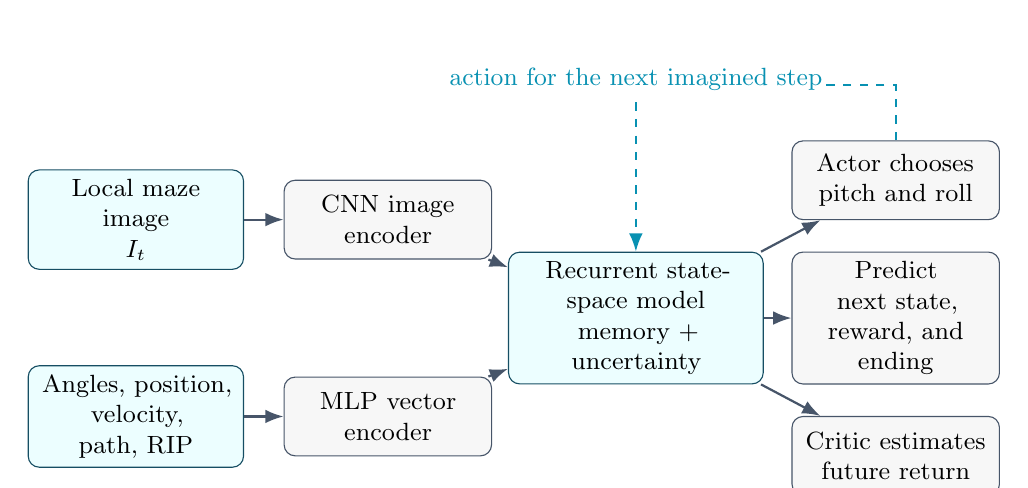
\begin{tikzpicture}[>=Latex,font=\small]
\tikzset{
input/.style={draw=tagblue,rounded corners,fill=taglight,text width=25mm,minimum height=11mm,align=center},
block/.style={draw=taggray,rounded corners,fill=gray!6,text width=24mm,minimum height=10mm,align=center},
model/.style={draw=tagblue,rounded corners,fill=taglight,text width=30mm,minimum height=16mm,align=center},
a/.style={->,thick,color=taggray},
imag/.style={->,thick,dashed,color=tagcyan}}

\node[input] (image) at (0,1.25) {Local maze image\\$I_t$};
\node[input] (vector) at (0,-1.25) {Angles, position,\\velocity, path, RIP};
\node[block] (cnn) at (3.2,1.25) {CNN image\\encoder};
\node[block] (mlp) at (3.2,-1.25) {MLP vector\\encoder};
\node[model] (rssm) at (6.35,0) {Recurrent state-space model\\memory + uncertainty};
\node[block] (actor) at (9.65,1.75) {Actor chooses\\pitch and roll};
\node[block] (heads) at (9.65,0) {Predict next state,\\reward, and ending};
\node[block] (critic) at (9.65,-1.75) {Critic estimates\\future return};

\draw[a] (image)--(cnn);
\draw[a] (vector)--(mlp);
\draw[a] (cnn)--(rssm);
\draw[a] (mlp)--(rssm);
\draw[a] (rssm)--(actor);
\draw[a] (rssm)--(heads);
\draw[a] (rssm)--(critic);

% During an imagined rollout, the actor's action becomes an input to the
% world model at the next imagined step. Route this feedback above all boxes
% so the label remains horizontal and does not overlap any node.
\draw[imag] (actor.north) -- ++(0,0.70) -| node[pos=0.53,above,fill=white,inner sep=1.5pt]
{action for the next imagined step} (rssm.north);
\end{tikzpicture}
\caption{The main neural-network blocks used by DreamerV3 in TAG. The recurrent world model remembers recent motion. During imagination, the actor selects an action, the world model predicts what may happen next, and the critic estimates the future return.}
\label{fig:network}
\end{figure}

\textbf{Image encoder.} A Convolutional Neural Network (CNN) reads the small maze image. Convolution filters are useful here because the same wall, corner, or hole pattern can appear at different image locations. The CNN compresses the image into a shorter feature vector instead of passing every pixel directly to the controller.

\textbf{Vector encoder.} A Multi-Layer Perceptron (MLP) reads the measured values: board angle, marble position, marble velocity, path points, progress, previous action, and optional pendulum data. An MLP is suitable because these inputs already have clear numerical meanings.

\textbf{Recurrent world model.} The core memory is a Recurrent State-Space Model (RSSM). ``Recurrent'' means that it carries a hidden memory from one control step to the next. This memory helps represent information that is not fully visible in a single camera frame, such as marble momentum, servo delay, a recent wall impact, or the phase of the pendulum disturbance. The RSSM combines a deterministic recurrent state with a stochastic latent state. The deterministic part stores a running summary of the past. The stochastic part allows the model to represent uncertainty when several futures are possible~\cite{hafner2025dreamerv3}.

\textbf{Prediction heads.} Small MLP heads predict the next latent state, reward, and whether the episode is likely to continue. During training, the model also learns to reconstruct or explain the observation. These predictions create the ``world model'' used for imagined rollouts.

\textbf{Actor and critic.} The actor is an MLP that outputs a probability distribution for the two continuous pitch and roll actions. The critic is another MLP that estimates the future reward expected from the current latent state. DreamerV3 trains these two networks on trajectories generated inside the learned world model, so one real transition can support more than one policy update.

\subsection{Why we do not use a Transformer now}
A Transformer could also be used as the temporal model, and it may become useful when TAG is trained on many maps and much larger datasets. We do not use one in the current system for four practical reasons.

First, the recurrent RSSM is already part of DreamerV3 and has been tested for continuous-control tasks. It updates one compact hidden state at every step, which fits an online robot loop. Second, TAG already provides marble velocity and short path context, so the controller does not need to search through a very long history for basic motion information. Third, a Transformer attends to a sequence of earlier tokens. This can improve long-range memory, but its computation and memory grow with the context length, while recurrent models are efficient during step-by-step imagination~\cite{deng2023backbones}. Fourth, our real dataset is still small compared with the large and diverse datasets where Transformers are usually most useful.

This does not mean that a Transformer is always worse. Research has shown that Transformer world models can help some long-horizon problems, but the architecture must be designed carefully; a standard Transformer does not automatically produce better policy gradients~\cite{ma2024transformer}. For an undergraduate project, the recurrent DreamerV3 model gives us a simpler and better-tested starting point. A fair future study could keep the same TAG observations and replay data, then compare RSSM, Transformer, and possibly a structured state-space model using prediction error, success rate, inference time, and GPU memory.

\subsection{Reward and training}
The main reward is progress along a numbered path. A one-time bonus is given when the marble reaches a new checkpoint. Falling into a hole ends the episode with a penalty. Timeout and stuck checks prevent the robot from running forever without useful movement. Anti-shortcut checks reject large path jumps that are caused by a detector error or by crossing through an invalid part of the map.

We first train with the pendulum motor disabled. This lets the policy learn the maze, gravity, friction, camera geometry, and servo delay. After the base policy works, we can fine-tune with the pendulum active. Compatible old replay should be kept because it still contains useful ball and board dynamics. New pendulum-active replay then teaches the extra disturbance.

\subsection{Why DreamerV3?}
No single controller is best for every part of TAG. We still use normal position control inside the servos. PID or LQR is useful for a known local target, but it does not decide how to move through a full maze with holes and impacts. Model Predictive Control is a strong alternative, but it needs a good model of rolling contact, friction, delay, and pendulum disturbance. PPO is easier to understand, but it does not reuse old physical data as strongly. SAC is an important model-free baseline because it is off-policy, but it still learns mainly from real replay transitions. DreamerV3 is attractive because it reuses replay and trains the policy using predicted future trajectories~\cite{hafner2025dreamerv3}. Its recurrent state is also a natural fit for hidden momentum, delay, and pendulum motion. The tradeoff is more software complexity and the risk of learning an inaccurate world model.

\callout{Practical reason for our choice.}{Physical data are expensive. Motors heat up, episodes may require resets, and unsafe exploration can drop the marble into a hole. DreamerV3 gives us a way to learn more from each real transition, while standard controllers remain responsible for the simple low-level loops.}

The maze-control formulation above provides the high-level roll and pitch commands. The next two sections describe the top-mounted Furuta mechanism and the separate continuous-control policy used to swing up and stabilize it.

\section{Furuta Pendulum System}



\subsection{System Overview}

This contribution to TAG covers control of the top-mounted Furuta pendulum
while the labyrinth moves underneath it: swing the pendulum up and hold it
along true gravity-vertical while the base undergoes roll and pitch
motion.

The controller combines board-motion measurements, encoder states, and IMU
signals into a 12-dimensional observation. A TQC actor maps this
observation to a motor-voltage command, which drives either the MuJoCo
model or the physical Furuta pendulum.

\begin{figure}[h]
\centering
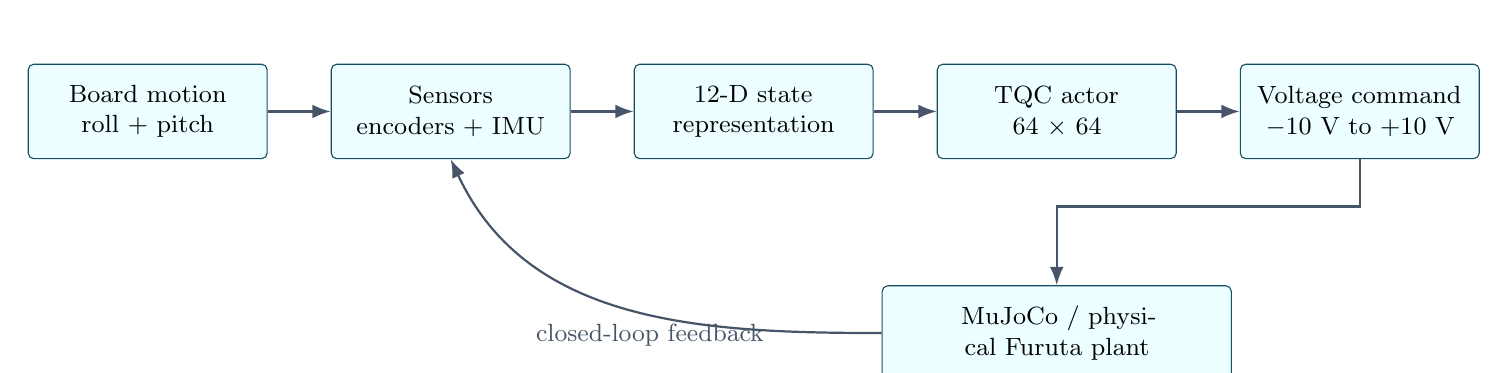
\begin{tikzpicture}[>=Latex,font=\small,node distance=8mm and 8mm]

\tikzset{
box/.style={
    draw=tagblue,
    rounded corners=2pt,
    fill=taglight,
    minimum height=12mm,
    text width=28mm,
    align=center
},
bigbox/.style={
    draw=tagblue,
    rounded corners=2pt,
    fill=taglight,
    minimum height=12mm,
    text width=42mm,
    align=center
},
arr/.style={->,thick,color=taggray}
}

\node[box] (motion) {Board motion\\roll + pitch};
\node[box, right=of motion] (sensor) {Sensors\\encoders + IMU};
\node[box, right=of sensor] (state) {12-D state\\representation};
\node[box, right=of state] (actor) {TQC actor\\64 $\times$ 64};
\node[box, right=of actor] (voltage) {Voltage command\\$-10$ V to $+10$ V};

\node[bigbox, below=16mm of actor] (plant) {MuJoCo / physical Furuta plant};

\draw[arr] (motion) -- (sensor);
\draw[arr] (sensor) -- (state);
\draw[arr] (state) -- (actor);
\draw[arr] (actor) -- (voltage);
\draw[arr] (voltage.south) -- ++(0,-6mm) -| (plant.north);

\draw[arr] (plant.west) to[out=180,in=-65] node[pos=0.45,below]{closed-loop feedback} (sensor.south);

\end{tikzpicture}
\caption{Pendulum-control workflow. Board motion and sensor measurements are
converted into a 12-dimensional state, the TQC actor produces a motor-voltage
command, and the resulting pendulum motion closes the feedback loop through the
plant and sensors.}
\label{fig:pendulum_workflow}
\end{figure}

% ============================================================
% PENDULUM CONTROL: STATE, OBSERVATION, AND SIMULATION
% ============================================================

\subsection{Pendulum State and Observation}

The Furuta pendulum has two joint coordinates: the rotary-arm angle
$\phi$, driven directly by the motor, and the pendulum angle $\theta$,
which rotates freely at the end of the arm. Their angular velocities,
$\dot{\phi}$ and $\dot{\theta}$, are also required, since balancing depends
on both position and motion.

\begin{figure}[h]
\centering

\includegraphics[width=0.43\linewidth]{pendulum model.png}
\caption{Furuta pendulum coordinates. The motor applies torque about the
rotary-arm axis $\phi$, while the pendulum rotates freely about the passive
joint with angle $\theta$.}
\label{fig:furuta_states}
\end{figure}

\subsubsection{Observation}

The final delay-robust controller uses a 12-dimensional observation:

\begin{equation}
\mathbf{s}_t =
\left[
\cos\theta_t,\;
\sin\theta_t,\;
\frac{\dot{\theta}_t}{15},\;
\frac{\phi_t}{\pi},\;
\frac{\dot{\phi}_t}{25},\;
a_{t-1},\;
\frac{r_t}{15^\circ},\;
\frac{p_t}{15^\circ},\;
\frac{\omega_{x,t}}{80^\circ/\mathrm{s}},\;
\frac{\omega_{y,t}}{80^\circ/\mathrm{s}},\;
a_{t-2},\;
a_{t-3}
\right].
\label{eq:pendulum_observation}
\end{equation}

The first five terms describe the Furuta pendulum itself. Roll $r$, pitch
$p$, and the board angular rates $\omega_x$ and $\omega_y$ describe the
motion of the moving base. The final three terms store recent motor
commands so the policy can account for actuator delay.

Encoding the pendulum angle as $\sin\theta$ and $\cos\theta$ avoids the
discontinuity that occurs when the angle wraps between $+\pi$ and $-\pi$.

The divisions in Eq.~\eqref{eq:pendulum_observation} are normalization
constants that scale quantities of different units and physical ranges into
similar numerical magnitudes before they reach the network — for example,
an arm velocity of roughly $25~\mathrm{rad/s}$ becomes a normalized value
near 1. This improves numerical conditioning during training and keeps the
preprocessing identical to what runs on the embedded controller.


% ============================================================

\subsection{Simulation Model}

A MuJoCo simulation reproduces the Furuta pendulum mounted on the two-axis
moving labyrinth, including the mechanical Furuta model, roll and pitch
motion of the base, joint sensors, board IMU measurements, and the
non-ideal behavior of the rotary-arm actuator.

\subsection{Joint Sensors}

The pendulum angle is measured with an \textbf{AS5600 magnetic absolute
encoder}, which provides 4096 counts per revolution. Calibration uses raw
value 2756 at the hanging position and 708 at the upright position, giving
exactly 2048 counts, or $180^\circ$, between the two configurations.

The rotary-arm angle is measured separately with an \textbf{AS5048A
magnetic encoder} over SPI. Together these encoders provide $\theta$,
$\phi$, and their corresponding angular velocities for the controller
observation.


% ============================================================
\subsection{Moving-Board IMU}

Board orientation and angular rate are measured with a
\textbf{SparkFun BNO086}. The controller uses board roll, pitch, and the
corresponding calibrated gyro measurements.

Hardware characterization measured the IMU's update rate, static
orientation noise, drift, rate scaling, and timing, and these measured
properties were reproduced in simulation rather than handing the controller
perfect MuJoCo states.

\begin{table}[h]
\centering
\small
\caption{Measured BNO086 characteristics used for simulation modeling.}
\begin{tabularx}{0.78\linewidth}{>{\bfseries}X X}
\toprule
Measured quantity & Result \\
\midrule
Controller loop rate & approximately $199.7$ Hz \\
BNO086 report rate & $99.7$--$100.0$ Hz \\
Roll static standard deviation & $0.0009^\circ$ \\
Pitch static standard deviation & $0.0116^\circ$ \\
Roll drift over 60 s & $-0.0005^\circ$ \\
Pitch drift over 60 s & $+0.0056^\circ$ \\
Measured rate scale & $0.986$--$1.001$ \\
Orientation lag relative to gyro & $2$--$3$ ms \\
Maximum tested physical board rate & approximately $92^\circ/\mathrm{s}$ \\
\bottomrule
\end{tabularx}
\end{table}

The simulated BNO086 therefore runs at roughly 100 Hz while the control
loop runs near 200 Hz, producing sample-and-hold behavior between IMU
updates. Orientation noise, gyro noise, bias, and timing delay are all
included in the simulated measurement path.


% ============================================================
\subsection{Actuator Model and System Identification}

The rotary arm is driven by the project BLDC/gimbal motor through a
TMC6300 driver using open-loop field-oriented control. Motor behavior was
identified experimentally with constant-voltage terminal-speed tests and
short initial-acceleration tests.

\begin{table}[h]
\centering
\small
\caption{Identified rotary-arm actuator parameters.}
\begin{tabularx}{0.78\linewidth}{>{\bfseries}X X}
\toprule
Parameter & Identified value \\
\midrule
Motor gain $K_M$ & $0.0127~\mathrm{N\,m/V}$ \\
Arm inertia $J_{\mathrm{arm}}$ & $6.5\times10^{-5}~\mathrm{kg\,m^2}$ \\
Viscous damping $b_\phi$ & $6.5\times10^{-4}~\mathrm{N\,m\,s/rad}$ \\
Effective back-EMF $K_E$ & $0.052~\mathrm{V\,s/rad}$ \\
Coulomb friction & approximately $6.85~\mathrm{mN\,m}$ \\
Breakaway voltage & approximately $0.15$--$0.237$ V \\
Speed at $\pm0.6$ V & approximately $9.4~\mathrm{rad/s}$ \\
Speed at $\pm1$ V & approximately $19~\mathrm{rad/s}$ \\
Speed at $\pm2$ V & approximately $25$--$29~\mathrm{rad/s}$ \\
Initial acceleration at $+6$ V & approximately $632~\mathrm{rad/s^2}$ \\
\bottomrule
\end{tabularx}
\end{table}

The TQC actor produces a normalized action $a_t\in[-1,1]$, converted into a
motor-voltage command:

\begin{equation}
\boxed{
V_{\mathrm{cmd},t}=V_{\max}a_t
}
\label{eq:voltage_command}
\end{equation}

where $V_{\max}=10$ V for the selected deployment policy. Before reaching
the simulated motor, the command passes through the identified actuator
chain:

\begin{center}
\textbf{
action $\rightarrow$ voltage command $\rightarrow$ delay
$\rightarrow$ slew-rate limit $\rightarrow$ motor lag
$\rightarrow$ Furuta plant
}
\end{center}

The resulting motor voltage is converted into rotary-arm torque using the
identified motor and friction parameters:

\begin{equation}
\boxed{
\tau_t =
K_M V_{\mathrm{motor},t}
-
K_E\dot{\phi}_t
-
b_\phi\dot{\phi}_t
-
\tau_c\,\mathrm{sgn}(\dot{\phi}_t)
}
\label{eq:actuator_torque}
\end{equation}

where $K_M$ is the motor gain, $K_E$ the effective back-EMF, $b_\phi$ the
viscous damping, and $\tau_c$ the Coulomb friction.

The control period is approximately $5$ ms. System identification also
found roughly $15$ ms of step-response dead time and a motor time constant
near $10$ ms, both included in simulation so the policy is not trained
against an unrealistically instantaneous motor.

% ============================================================
% REINFORCEMENT-LEARNING CONTROLLER
% ============================================================

\section{Reinforcement Learning for Pendulum Control with TQC}

\subsection{Why Reinforcement Learning?}

The Furuta pendulum is nonlinear and underactuated: only the rotary arm is
driven, while the pendulum moves freely. The controller must first inject
enough energy to swing the pendulum upward, then switch behavior to
stabilize the unstable upright equilibrium.

Classical methods can solve pieces of this problem — an energy-based
controller for swing-up, LQR or PID for stabilization near upright — but
this generally requires separate controllers, switching logic between
them, and an accurate model or local linearization. The moving-board
configuration adds further difficulty, since roll and pitch disturbances
continuously change the dynamics the pendulum experiences, on top of
friction, actuator saturation, motor delay, and sensor latency.

Reinforcement learning was chosen instead to learn a single nonlinear
policy,

\begin{equation}
s_t \longrightarrow \pi(s_t) \longrightarrow a_t,
\end{equation}

mapping the current observation $s_t$ directly to a continuous motor
command $a_t$. During training, the controller is exposed directly to
moving-board disturbances, sensor effects, actuator dynamics, and model
uncertainty, so all of these are handled by one learned policy rather than
switching logic.

\subsection{Why Truncated Quantile Critics?}

The selected algorithm is \textbf{Truncated Quantile Critics (TQC)}, a
model-free, off-policy actor--critic method for continuous-action control
that fits the Furuta system naturally, since the policy produces a
continuous action $a_t \in [-1,1]$ that is later converted to the commanded
motor voltage. Being model-free, TQC learns directly from sampled
transitions and never builds or consults an explicit dynamics model — all
of the plant's nonlinearity, board disturbance, and actuator behavior is
captured implicitly through interaction with the (randomized) simulator
rather than through an analytic approximation.

TQC has two main network components:

\begin{itemize}
    \item \textbf{Actor:} receives the normalized observation and produces
    the motor action.
    \item \textbf{Critics:} evaluate whether a state--action pair is likely
    to produce good long-term behavior.
\end{itemize}

The actor is a fully-connected multilayer perceptron (MLP) with two hidden
layers of 64 units each and ReLU activations. Its output head parameterizes
a tanh-squashed Gaussian over the action, so the sampled action is bounded
within $[-1,1]$ by construction rather than by post-hoc clipping. This is
the network that eventually runs on the embedded controller; the critics
are used only during training.\footnote{In plain terms: the actor is a
small neural network that uses ReLU nonlinearities so it can learn
non-linear relationships instead of just straight lines. During training
its output is a small random spread (Gaussian) around a mean action, which
lets the policy explore instead of always doing the same thing; this is
squashed through tanh so the sampled value always lands in $[-1,1]$,
matching the motor voltage range. Once training is done, only the mean is
used (no more randomness), and the critics are discarded — they only
existed to produce a learning signal, not to run on hardware.}

\begin{figure}[h]
\centering
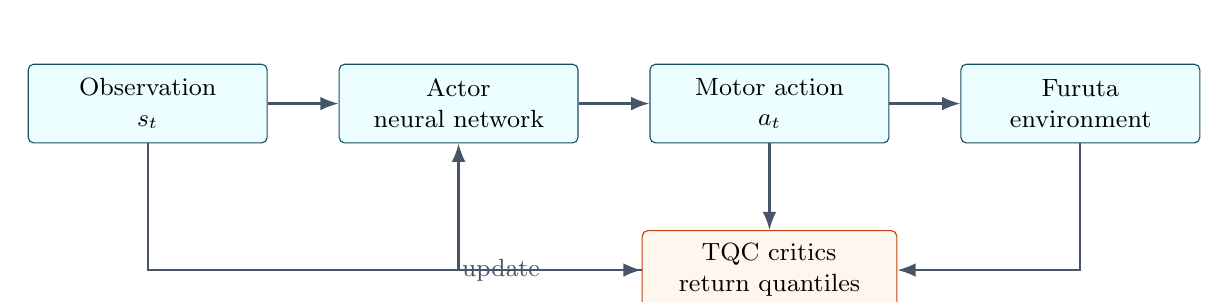
\begin{tikzpicture}[node distance=7mm and 9mm,>=Latex,font=\small]

\tikzset{
b/.style={
    draw=tagblue,
    rounded corners=2pt,
    fill=taglight,
    minimum height=10mm,
    text width=28mm,
    align=center
},
critic/.style={
    draw=tagorange,
    rounded corners=2pt,
    fill=orange!7,
    minimum height=10mm,
    text width=30mm,
    align=center
},
a/.style={->,thick,color=taggray}
}

\node[b] (state) {Observation\\$s_t$};
\node[b,right=of state] (actor) {Actor\\neural network};
\node[b,right=of actor] (action) {Motor action\\$a_t$};
\node[b,right=of action] (plant) {Furuta\\environment};

\node[critic,below=11mm of action] (critics)
{TQC critics\\return quantiles};

\draw[a] (state) -- (actor);
\draw[a] (actor) -- (action);
\draw[a] (action) -- (plant);

\draw[a] (state.south) |- (critics.west);
\draw[a] (action.south) -- (critics.north);
\draw[a] (plant.south) |- (critics.east);

\draw[a] (critics.west) -| node[pos=0.25,left]{update} (actor.south);

\end{tikzpicture}
\caption{Actor--critic structure used during TQC training. The actor selects
the motor command, while the critics estimate its long-term value and
provide the learning signal used to improve the actor.}
\label{fig:tqc_structure}
\end{figure}


% ============================================================
\subsection{What Does the Critic Predict?}

The critic does not judge an action solely on the reward it produces
immediately. A motor command may momentarily push the pendulum toward
upright while also imparting excessive angular velocity that causes a fall
several steps later. So instead, the critic estimates the \textbf{return}
— the total reward the agent expects to collect from this point until the
episode ends, not just the reward from the current action:

\begin{equation}
\boxed{
G_t =
r_t
+
\gamma r_{t+1}
+
\gamma^2 r_{t+2}
+
\gamma^3 r_{t+3}
+\cdots
}
\label{eq:return}
\end{equation}

where $r_t$ is the immediate reward and $\gamma\in(0,1)$ is the discount
factor. Judging an action only by $r_t$ can be misleading: pushing the
pendulum toward upright may look good this instant, but if that same push
also imparts a large angular velocity, the pendulum overshoots and falls a
moment later — a poor outcome that $r_t$ alone would miss. The return
folds in those later consequences by summing all future rewards, with
$\gamma$ discounting rewards further in the future so the sum stays finite
and near-term consequences are weighted more heavily than distant ones.
The critic's job is to predict this return for a given state and action
before the episode actually plays out, and that prediction is what teaches
the actor which actions are genuinely good rather than merely good in the
moment.

For example, of two actions near the upright position, one may give a
similar immediate reward but let the pendulum fall shortly after, while the
other keeps it stable. The critic should assign the second a larger value,
since it produces a larger long-term return.

A conventional critic estimates the expected return
$Q(s_t,a_t) \approx \mathbb{E}[G_t]$. TQC instead predicts multiple
quantiles of the return distribution,
$Z(s_t,a_t) = \{z_1,z_2,\ldots,z_N\}$, and discards the largest predicted
quantiles when constructing the critic target. This truncation reduces
optimistic value estimation and lowers the chance that the actor learns an
aggressive action only because its future value was overestimated.

After training, the critics are no longer needed — real-time control uses
only

\begin{equation}
\boxed{
\text{observation}
\longrightarrow
\text{actor}
\longrightarrow
\text{motor command}.
}
\end{equation}


% ============================================================
\subsection{Reward and Cost Design}

The objective is not simply to pass through the upright position. The
controller should swing the pendulum up, capture it, hold it aligned with
true gravity vertical under board motion, avoid excessive rotary-arm
motion, and issue smooth, hardware-compatible commands. For documentation,
the implemented reward is equivalently represented as the stage cost

\begin{align}
J_t ={}&
\underbrace{(1-u_t)}_{\text{upright error}}
+
\underbrace{w_{\phi}
\left(\frac{\phi_t}{\pi}\right)^2}_{\text{arm centering}}
+
\underbrace{0.005a_t^2}_{\text{control effort}}
\notag\\
&+
\underbrace{0.002\dot{\phi}_t^2}_{\text{arm velocity}}
+
\underbrace{w_{\Delta a}
(a_t-a_{t-1})^2}_{\text{action smoothness}}
\notag\\
&+
\underbrace{
0.01\,\mathbb{I}(u_t>0.5)\dot{\theta}_t^2
}_{\text{pole settling}}
+
\underbrace{P_{\mathrm{arm}}(\phi_t)}_{\text{arm envelope}}
+
\underbrace{P_{\mathrm{cable}}(\phi_t)}_{\text{cable safety}}
-
\underbrace{B_{\mathrm{upright}}}_{\text{stable-balance bonus}} .
\label{eq:pendulum_cost}
\end{align}

The RL environment maximizes the corresponding reward, so lower cost in
Eq.~\eqref{eq:pendulum_cost} means better control behavior.

\subsubsection*{World-frame uprightness}

The primary objective is alignment with gravity vertical:

\begin{equation}
u_t =
\hat{\mathbf z}_{\mathrm{pole}}^{T}
\hat{\mathbf z}_{\mathrm{world}}
=
\cos(e_t),
\label{eq:uprightness}
\end{equation}

where $e_t$ is the angular error from true vertical, so
$u_t=1$ upright, $u_t=0$ horizontal, $u_t=-1$ downward. This definition
matters because board tilt does not redefine the target direction — even
as the board rolls or pitches, the target stays aligned with gravity.

\begin{table}[h]
\centering
\small
\caption{Physical interpretation of the cost terms.}
\begin{tabularx}{0.96\linewidth}
{>{\bfseries}p{0.25\linewidth} X}
\toprule
Cost term & Purpose \\
\midrule

$1-u_t$
&
Primary objective. Penalizes deviation of the pendulum from true vertical.
\\

$w_{\phi}(\phi_t/\pi)^2$
&
Discourages unnecessary rotary-arm displacement and keeps the arm in a
practical operating region.
\\

$0.005a_t^2$
&
Penalizes unnecessarily large motor commands.
\\

$0.002\dot{\phi}_t^2$
&
Discourages excessive rotary-arm velocity.
\\

$w_{\Delta a}(a_t-a_{t-1})^2$
&
Penalizes rapid changes between consecutive actions, encouraging smoother
motor commands.
\\

$0.01\,\mathbb{I}(u_t>0.5)\dot{\theta}_t^2$
&
Penalizes pendulum angular velocity only near upright, allowing the
pendulum to build energy during swing-up while encouraging settling during
capture.
\\

$P_{\mathrm{arm}}$
&
Soft penalty for leaving the preferred rotary-arm operating region.
\\

$P_{\mathrm{cable}}$
&
Penalizes motion near the physical cable limit.
\\

$-B_{\mathrm{upright}}$
&
Rewards stable balancing when the pendulum is tightly upright and the arm
remains in the safe region.
\\

\bottomrule
\end{tabularx}
\end{table}


% ============================================================
\subsubsection*{Swing-up and Stabilization Behavior}

A particularly important term is the conditional pendulum-velocity cost:

\begin{equation}
J_{\dot{\theta}} =
\begin{cases}
0,
& u_t \leq 0.5,\\[1mm]
0.01\dot{\theta}_t^2,
& u_t > 0.5.
\end{cases}
\label{eq:pole_velocity_cost}
\end{equation}

During swing-up the pendulum needs angular velocity to gain energy, so
penalizing $\dot{\theta}$ throughout the episode would fight the desired
motion. Once the pendulum nears upright, however, large angular velocity
becomes undesirable, since the controller must capture and settle it. The
conditional term therefore switches the preferred behavior naturally:

\begin{center}
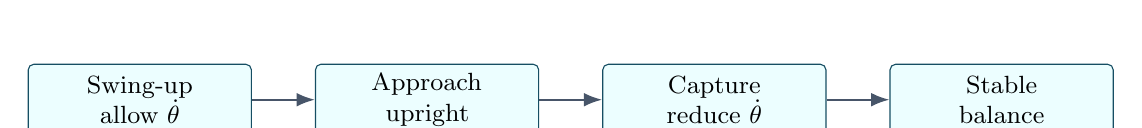
\begin{tikzpicture}[node distance=7mm and 8mm,>=Latex,font=\small]

\tikzset{
b/.style={
    draw=tagblue,
    rounded corners=2pt,
    fill=taglight,
    minimum height=9mm,
    text width=26mm,
    align=center
},
a/.style={->,thick,color=taggray}
}

\node[b] (swing) {Swing-up\\allow $\dot{\theta}$};
\node[b,right=of swing] (approach) {Approach\\upright};
\node[b,right=of approach] (capture) {Capture\\reduce $\dot{\theta}$};
\node[b,right=of capture] (balance) {Stable\\balance};

\draw[a] (swing) -- (approach);
\draw[a] (approach) -- (capture);
\draw[a] (capture) -- (balance);

\end{tikzpicture}
\end{center}

The complete reward thus encourages a sequence of behaviors rather than a
single static objective:

\begin{equation}
\boxed{
\text{swing up}
\rightarrow
\text{capture}
\rightarrow
\text{stabilize}
\rightarrow
\text{reject board disturbance}.
}
\end{equation}
% ============================================================
% TRANSFER LEARNING AND CATASTROPHIC FORGETTING
% ============================================================

\section{Coupled Board--Pendulum Dynamics and Vibration}
The maze-control and Furuta-pendulum subsystems are physically coupled because the pendulum base is mounted directly on the TAG board. Motion of the rotary arm and pendulum produces reaction forces and torques that pass through the mounting structure into the labyrinth. These disturbances can change the instantaneous board orientation and can introduce vibration into the marble-control task in addition to the commanded roll and pitch motion.

The coupling is bidirectional. Pendulum motion disturbs the board and therefore the marble, while roll and pitch of the TAG platform change the orientation of gravity relative to the moving pendulum base. The two learned controllers must therefore be evaluated as parts of a common mechanical system rather than only as independent tasks.

\subsection{Reaction Forces and Torques}
Motion of the rotary arm generates an equal and opposite reaction torque on the pendulum base. Because the base is rigidly connected to the TAG board, that reaction is transmitted to the board through the mechanical mounting and the simulated rigid-body constraints. The interaction can be summarized conceptually as
\begin{equation}
\tau_m
\rightarrow
\ddot{\phi}
\rightarrow
\tau_{\mathrm{reaction}}
\rightarrow
\text{board motion}
\rightarrow
\text{marble motion}.
\end{equation}
The same physics path provides a direct way to measure joint reactions and board motion in an integrated simulator before comparing them with board-IMU data from the physical platform.

\subsection{Board Vibration}
Rigid-body reaction motion captures the lower-frequency disturbance created by arm and pendulum acceleration. The physical assembly can also generate higher-frequency vibration through motor rotation, rotor imbalance, bearings, structural flexibility, mounting compliance, and rapid changes in pendulum acceleration. The first integrated model therefore allows vibration to arise naturally from the coupled dynamics. Measured disturbances can later be added through calibrated compliance, damping, and motor-imbalance models instead of prescribing arbitrary board motion.

To resolve these effects, the simulation time step must be sufficiently smaller than the vibration period, and the board joints must retain physically meaningful stiffness and damping rather than behaving as perfectly rigid kinematic constraints. Pendulum mass and inertia, board inertia, joint damping, actuator response, and mounting stiffness are therefore central calibration quantities for coupled simulation and sim-to-real transfer.

\section{Pendulum Control on a Moving Board}

The Furuta assembly sits on a nested two-axis gimbal: one joint produces
roll, the second produces pitch. The actuated rotary arm and passive
pendulum are attached to this moving frame, so MuJoCo computes the coupled
effects of gravity, inertia, board motion, friction, and joint damping
together.

Board motion is treated purely as an external disturbance — the pendulum
controller acts only through the rotary-arm motor and does not command the
labyrinth's roll or pitch. The simulated board is mechanically limited to
roughly $\pm 15^\circ$ in both roll and pitch, and continuous disturbance
trajectories are used rather than instantaneous angle changes so the
simulated base has realistic angular velocity and acceleration.

\begin{table}[h]
\centering
\small
\caption{Moving-board parameters used during training and verification.}
\begin{tabularx}{0.78\linewidth}{>{\bfseries}X X}
\toprule
Quantity & Value \\
\midrule
Roll limit & $\pm 15^\circ$ \\
Pitch limit & $\pm 15^\circ$ \\
Maximum diagonal tilt & approximately $21.1^\circ$ \\
Production-training range & approximately $\pm 10^\circ$ \\
Production-training speed cap & $60^\circ/\mathrm{s}$ \\
Final verification speed & up to $120^\circ/\mathrm{s}$ \\
High-speed acceleration bound & $1200^\circ/\mathrm{s}^2$ \\
\bottomrule
\end{tabularx}
\end{table}


% ============================================================

\subsection{Curriculum Training under Board Motion}

Training directly under the hardest two-axis board motion can destabilize
the transferred policy and make exploration inefficient, so a curriculum
increases task difficulty progressively:

\begin{equation}
\boxed{
\text{Train at current difficulty}
\rightarrow
\text{Evaluate}
\rightarrow
\text{Increase difficulty when reliable}
}
\end{equation}

The controller begins from the transferred swing-up and balancing policy.
Moving-base disturbances are then introduced gradually — early stages use
milder roll and pitch motion so the actor can learn the effect of base
motion without immediately losing behavior it already learned. As
performance improves, disturbance magnitude, board speed, and task
complexity increase until the final two-axis operating condition is
reached.

\begin{figure}[h]
\centering
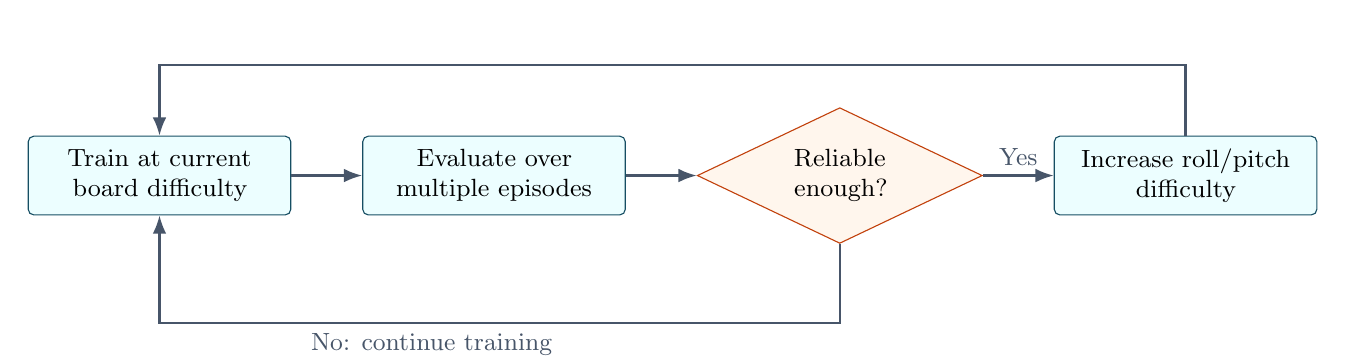
\begin{tikzpicture}[node distance=8mm and 9mm,>=Latex,font=\small]

\tikzset{
stage/.style={
    draw=tagblue,
    rounded corners=2pt,
    fill=taglight,
    minimum height=10mm,
    text width=31mm,
    align=center
},
decision/.style={
    diamond,
    draw=tagorange,
    fill=orange!7,
    aspect=2.1,
    text width=20mm,
    align=center,
    inner sep=1pt
},
arrow/.style={->,thick,color=taggray}
}

\node[stage] (train) {Train at current\\board difficulty};
\node[stage,right=of train] (eval) {Evaluate over\\multiple episodes};
\node[decision,right=of eval] (reliable) {Reliable\\enough?};
\node[stage,right=of reliable] (increase) {Increase roll/pitch\\difficulty};

\draw[arrow] (train) -- (eval);
\draw[arrow] (eval) -- (reliable);
\draw[arrow] (reliable) -- node[above]{Yes} (increase);

\draw[arrow]
(reliable.south)
-- ++(0,-10mm)
-| node[pos=0.30,below]{No: continue training}
(train.south);

\draw[arrow]
(increase.north)
-- ++(0,9mm)
-| (train.north);

\end{tikzpicture}

\caption{Curriculum-training loop. The policy remains at the current
difficulty until evaluation indicates sufficient reliability, after which
the moving-board disturbance is increased.}
\label{fig:curriculum_training}
\end{figure}

The overall progression is

\begin{equation}
\boxed{
\begin{array}{c}
\text{Pretrained Swing-up and Balance Policy}\\
\downarrow\\
\text{Mild Moving-Board Disturbance}\\
\downarrow\\
\text{Larger Roll/Pitch Motion}\\
\downarrow\\
\text{Faster Two-Axis Motion}\\
\downarrow\\
\text{Robustness and Domain Randomization}\\
\downarrow\\
\text{Final Two-Axis Policy}
\end{array}
}
\end{equation}

This curriculum serves two purposes: it reduces the difficulty of
exploration, since the controller does not need to learn swing-up,
stabilization, and strong disturbance rejection all at once, and it reduces
the risk of catastrophic forgetting, since each stage is only a moderate
change from the behavior learned in the previous one.
% ============================================================
% SIM-TO-REAL TRANSFER
% ============================================================

\section{Sim-to-Real Transfer}

\subsection{Transfer Learning and Catastrophic Forgetting}

The moving-board controller was not trained from scratch. A previously
trained policy already had useful swing-up and balancing behavior, so the
next training stage aimed to preserve that behavior while learning to
reject the additional disturbances from board motion:

\begin{equation}
\boxed{
\text{Swing-up + Balance}
\;\longrightarrow\;
\text{Swing-up + Balance + Moving-board Robustness}
}
\end{equation}

\subsubsection{Catastrophic Forgetting}

During fine-tuning, the actor is updated using experience from the new
moving-board environment. If the policy changes too aggressively, it can
improve disturbance rejection while losing previously learned swing-up,
capture, or balancing behavior — a failure mode known as
\textbf{catastrophic forgetting}. The goal of transfer learning is to adapt
the previous controller without unnecessarily destroying behavior that
already works.

\subsubsection{Actor Transfer and Critic Reset}

The actor and critics play different roles and are treated accordingly.
The \textbf{actor} is retained, since it already contains useful control
behavior: $\pi_{\mathrm{old}} \rightarrow \pi_{\mathrm{new}}$. The previous
critics, however, estimate future return for the earlier environment, and
once board motion, new disturbances, and additional observations are
introduced, those value estimates are no longer trustworthy. The transfer
strategy is therefore

\begin{equation}
\boxed{
\begin{array}{ccc}
\text{Previous Actor} & \longrightarrow & \text{Retain} \\
\text{Previous Critics} & \longrightarrow & \text{Reset}
\end{array}}
\end{equation}

This preserves the previously learned motor-control behavior while letting
the value function be relearned for the new moving-board task.

\subsubsection{Critic Warm-Up}

Immediately after the critic reset, the new critics do not yet provide
reliable return estimates, and updating the actor from these inaccurate
values could quickly damage the transferred policy. The actor is therefore
temporarily frozen while the new critics learn from experience generated by
the transferred policy.

\begin{center}
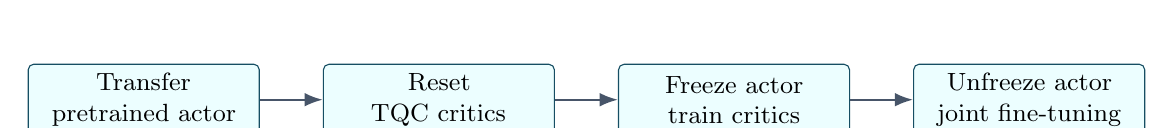
\begin{tikzpicture}[node distance=7mm and 8mm,>=Latex,font=\small]

\tikzset{
b/.style={
    draw=tagblue,
    rounded corners=2pt,
    fill=taglight,
    minimum height=9mm,
    text width=27mm,
    align=center
},
a/.style={->,thick,color=taggray}
}

\node[b] (transfer) {Transfer\\pretrained actor};
\node[b,right=of transfer] (reset) {Reset\\TQC critics};
\node[b,right=of reset] (freeze) {Freeze actor\\train critics};
\node[b,right=of freeze] (joint) {Unfreeze actor\\joint fine-tuning};

\draw[a] (transfer) -- (reset);
\draw[a] (reset) -- (freeze);
\draw[a] (freeze) -- (joint);

\end{tikzpicture}
\end{center}

During warm-up, the transferred actor continues generating actions while
the critics learn the return distribution of the new environment. Once the
critics give a useful learning signal, the actor is unfrozen and allowed to
adapt.

\subsubsection{Policy Retention}

The previous actor can also be kept as a teacher, or reference policy,
during fine-tuning to discourage unnecessary changes to behavior that
already works:

\begin{equation}
\boxed{
L_{\mathrm{ret}}
=
\left\|
\pi_{\mathrm{new}}(s)
-
\pi_{\mathrm{teacher}}(s)
\right\|^2
}
\label{eq:retention_loss}
\end{equation}

A large difference between the new and teacher actions increases this
loss. It does not prevent the new actor from adapting to board motion — it
simply discourages unnecessary changes when the previous behavior still
works.

The overall transfer-learning procedure can be summarized as

\begin{equation}
\boxed{
\text{Pretrained Policy}
\rightarrow
\text{Retain Actor}
\rightarrow
\text{Reset Critics}
\rightarrow
\text{Critic Warm-Up}
\rightarrow
\text{Joint Fine-Tuning}
}
\end{equation}
% ============================================================
% CURRICULUM TRAINING
% ============================================================

Even after system identification, the MuJoCo model cannot reproduce the
physical Furuta system exactly — differences remain in motor strength,
friction, inertia, sensor noise, and control latency. A policy trained
against only one exact simulation can therefore overfit to that model and
perform poorly on hardware. The sim-to-real strategy combines three steps:

\begin{equation}
\boxed{
\text{System Identification}
\rightarrow
\text{Domain Randomization}
\rightarrow
\text{Hardware Deployment}
}
\end{equation}

\subsection{System Identification}

The nominal simulation model is built from measurements of the physical
system — motor gain, rotary-arm dynamics, pendulum friction, encoder
calibration, BNO086 measurements, and actuator timing are all identified
experimentally and reproduced in MuJoCo, reducing the initial gap between
simulation and hardware before robustness training begins.

\subsection{Domain Randomization}

The identified parameters are not assumed exact. During robustness
training, selected mechanical, sensor, and timing parameters are randomly
varied around their nominal values, so the policy learns to perform well
over a family of plausible systems rather than one exact simulated plant:

\begin{equation}
\pi^*
=
\pi^*
\left(
K_M,\,
b_\phi,\,
b_\theta,\,
J_p,\,
\tau_f,\,
\sigma_{\mathrm{obs}},\,
d_{\mathrm{act}}
\right),
\end{equation}

where the terms represent motor strength, joint damping, inertia, friction,
observation uncertainty, and actuator delay.

\begin{table}[h]
\centering
\footnotesize
\renewcommand{\arraystretch}{0.95}
\caption{Parameters randomized during robustness training.}
\begin{tabularx}{0.96\linewidth}
{>{\bfseries}p{0.28\linewidth}
 p{0.25\linewidth}
 X}
\toprule
Randomized parameter & Training range & Purpose \\
\midrule

Motor gain $K_M$
&
$0.010$--$0.016~\mathrm{N\,m/V}$
&
Accounts for uncertainty in motor strength and voltage-to-torque response.
\\

Arm viscous damping $b_\phi$
&
$3\times10^{-4}$--$1\times10^{-3}~
\mathrm{N\,m\,s/rad}$
&
Represents uncertainty in rotary-arm damping and bearing friction.
\\

Pendulum damping $b_\theta$
&
$1.4\times10^{-5}$--$5.4\times10^{-5}~
\mathrm{N\,m\,s/rad}$
&
Accounts for changes in passive pendulum-joint damping.
\\

Arm Coulomb friction
&
$4\times10^{-3}$--$8\times10^{-3}~\mathrm{N\,m}$
&
Represents uncertainty in dry friction at the rotary-arm joint.
\\

Pendulum Coulomb friction
&
$6.5\times10^{-5}$--$2.65\times10^{-4}~\mathrm{N\,m}$
&
Represents uncertainty in the passive pendulum bearing.
\\

Pendulum inertia
&
$0.92$--$1.08\times$ nominal
&
Accounts for uncertainty in mass distribution and inertia.
\\

Observation-angle noise
&
$0$--$0.01~\mathrm{rad}$
&
Prevents the policy from relying on perfectly measured joint angles.
\\

Action delay
&
$1$--$2$ control steps
&
Represents uncertainty in computation, communication, and actuator latency.
\\

Corner-condition probability
&
$0.10$
&
Increases exposure to difficult moving-board conditions.
\\

\bottomrule
\end{tabularx}
\end{table}

At the roughly $200~\mathrm{Hz}$ control rate, one control step is about
$5~\mathrm{ms}$, so the randomized one- to two-step action delay
corresponds to approximately $5$--$10~\mathrm{ms}$.

\FloatBarrier

\subsection{Progressive Robustness Training}

Domain randomization is introduced progressively rather than applying the
full parameter variation immediately, letting the controller retain its
nominal balancing behavior while gradually adapting to increasing model
uncertainty:

\begin{center}
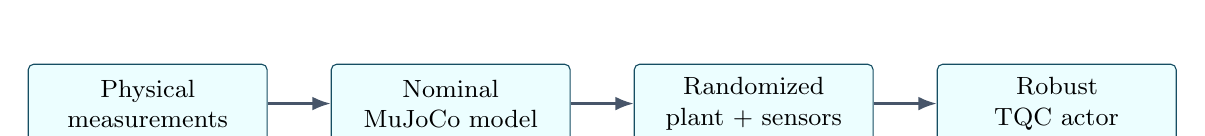
\begin{tikzpicture}[node distance=7mm and 8mm,>=Latex,font=\small]

\tikzset{
b/.style={
    draw=tagblue,
    rounded corners=2pt,
    fill=taglight,
    minimum height=10mm,
    text width=28mm,
    align=center
},
a/.style={->,thick,color=taggray}
}

\node[b] (measure) {Physical\\measurements};
\node[b,right=of measure] (nominal) {Nominal\\MuJoCo model};
\node[b,right=of nominal] (random) {Randomized\\plant + sensors};
\node[b,right=of random] (robust) {Robust\\TQC actor};

\draw[a] (measure) -- (nominal);
\draw[a] (nominal) -- (random);
\draw[a] (random) -- (robust);

\end{tikzpicture}
\end{center}

The resulting actor is therefore not optimized for one fixed set of
simulation parameters — it is trained to tolerate realistic variation
around the identified physical system.

\subsection{Sensor and Timing Matching}

Sim-to-real transfer also requires the timing of simulated measurements to
match the physical controller. The main control loop runs at roughly
$200~\mathrm{Hz}$, while the BNO086 provides orientation and gyro
measurements near $100~\mathrm{Hz}$; the simulation reproduces this gap
with sample-and-hold behavior, measurement noise, bias, and timing delay.
Actuator delay, motor lag, voltage saturation, and slew-rate limits are
likewise included during training, reducing the chance that the policy
learns high-frequency behavior only an ideal simulated actuator could
produce.

The overall sim-to-real pipeline is therefore

\begin{equation}
\boxed{
\text{Physical Measurements}
\rightarrow
\text{Nominal Simulation}
\rightarrow
\text{Domain Randomization}
\rightarrow
\text{Robust Actor}
\rightarrow
\text{Hardware Deployment}.
}
\end{equation}
% ============================================================
% POLICY DEPLOYMENT TO ESP32
% ============================================================

\section{Hardware Deployment}

Only the trained \textbf{actor network} is required for deployment — the
TQC critics improve the actor during training but are not needed for
real-time control:

\begin{equation}
\boxed{
\text{TQC Checkpoint}
\rightarrow
\text{Extract Actor}
\rightarrow
\text{C Header}
\rightarrow
\text{ESP32 Firmware}
\rightarrow
\text{Motor Command}
}
\end{equation}

The trained actor weights are exported from the Python checkpoint into a
C-compatible header file, and the same network is evaluated directly on
the ESP32. At each control step, the firmware:

\begin{enumerate}
    \item reads the AS5600 pendulum encoder;
    \item reads the AS5048A rotary-arm encoder;
    \item reads roll, pitch, and angular rates from the BNO086;
    \item constructs the observation using the same ordering used during
    training;
    \item applies the same normalization used in simulation;
    \item evaluates the actor neural network;
    \item converts the normalized action to the commanded motor voltage.
\end{enumerate}

The real-time control path is therefore

\begin{equation}
\boxed{
\text{Sensors}
\rightarrow
\text{12-D Observation}
\rightarrow
\text{Normalization}
\rightarrow
\text{Actor}
\rightarrow
a_t
\rightarrow
V_{\mathrm{cmd}}
}
\end{equation}

The controller runs at approximately $200~\mathrm{Hz}$, a control period of
roughly $5~\mathrm{ms}$.

\subsection{Deployment Verification}

Before enabling the motor, the exported actor is checked against the
original Python policy by passing the same observation through both
implementations and comparing outputs — this verifies that network
weights, activation functions, observation order, and normalization were
all exported correctly. A motor-disabled verification mode is also used
before powered testing, so the complete sensing and inference pipeline can
run with the motor disabled.

The main items checked before deployment:

\begin{itemize}
    \item encoder direction and zero reference;
    \item BNO086 roll and pitch sign conventions;
    \item observation ordering;
    \item observation normalization;
    \item actor output range;
    \item stale or invalid sensor handling.
\end{itemize}

Hardware testing then proceeds progressively, using a reduced motor voltage
before enabling the full deployment limit — a staged approach that reduces
the risk of a sign error, incorrect state normalization, or unexpected
actuator response producing a large motor command.


% ============================================================
% RESULTS
% ============================================================

\section{Experimental Results}

\subsection{Maze Navigation Results}

Figure~\ref{fig:training} shows one long TensorBoard run. The success rate stayed close to zero for most of training and then increased after about three million environment steps. The smoothed success-rate value shown at step 4,240,020 is 0.3792. Episode duration changed throughout training, and the smoothed log reward increased before dropping near the end. These plots show that the policy learned useful behavior, but they are not enough to make a final performance claim. The raw curves have large variation, and only one run is shown.

\begin{figure}[H]
\centering
\begin{subfigure}[t]{0.32\linewidth}
\centering

\includegraphics[width=\linewidth]{tag_success_rate.png}
\caption{Success rate over 100 episodes.}
\end{subfigure}\hfill
\begin{subfigure}[t]{0.32\linewidth}
\centering

\includegraphics[width=\linewidth]{tag_episode_duration.png}
\caption{Episode duration.}
\end{subfigure}\hfill
\begin{subfigure}[t]{0.32\linewidth}
\centering

\includegraphics[width=\linewidth]{tag_log_reward.png}
\caption{Cumulative log reward.}
\end{subfigure}
\caption{Preliminary TensorBoard curves from one baseline run at 4,240,020 environment steps. Dark lines are smoothed values. Final evaluation should use repeated runs and fixed starting positions.}
\label{fig:training}
\end{figure}

The next evaluation should report success rate, completion time, maximum progress, hole rate, and physical training steps. We also plan a small ablation study: the same configuration with and without measured marble velocity. This will show whether $(v_x,v_y)$ actually improves learning speed and stability.

\subsection{Pendulum Simulation and Moving-Board Results}

The final controller was evaluated on sustained balancing performance
rather than training reward alone: a successful episode requires the
pendulum to remain balanced for the required portion of the final
evaluation window without violating the configured failure conditions.

The selected policy uses a maximum motor command of $V_{\max}=10~\mathrm{V}$.
Under the hardest reported two-axis verification condition, the board
moved simultaneously in roll and pitch with $|r|,\;|p| \leq 15^\circ$ and
angular rates reaching approximately $120^\circ/\mathrm{s}$. At this
condition the selected policy achieved approximately

\begin{equation}
\boxed{
96\% \text{ sustained success}
}
\end{equation}

and at lower board-motion rates, sustained success remained approximately
$96$--$99\%$.

\begin{table}[h]
\centering
\small
\caption{Summary of the final simulated controller performance.}
\begin{tabularx}{0.82\linewidth}{>{\bfseries}X X}
\toprule
Quantity & Result \\
\midrule
Motor-voltage limit & $10~\mathrm{V}$ \\
Maximum tested roll & $\pm15^\circ$ \\
Maximum tested pitch & $\pm15^\circ$ \\
Maximum tested board rate & approximately $120^\circ/\mathrm{s}$ \\
Sustained success at hardest condition & approximately $96\%$ \\
Lower-speed sustained success & approximately $96$--$99\%$ \\
Control frequency & approximately $200~\mathrm{Hz}$ \\
\bottomrule
\end{tabularx}
\end{table}

Evaluation went beyond whether the pole briefly reached upright, also
checking rotary-arm travel, cable-limit violations, action saturation, and
robustness to parameter variation and actuator delay.

\subsection{Hardware Deployment Results}

The exported actor was successfully executed on the ESP32 using the same
state construction and normalization used during simulation. Hardware
bring-up demonstrated successful pendulum catches and balancing behavior on
the physical Furuta mechanism, though testing also showed that actuator
delay and motor dynamics were important sources of mismatch between ideal
simulation performance and hardware behavior. These observations motivated
adding actuator lag, delay-aware observations, and stronger robustness
testing to the simulation — the hardware results served not only as final
validation but also as feedback for improving the simulation model and
training procedure.


% ============================================================
% CONCLUSION
% ============================================================

\section{Generalization Across Maze Configurations}

A long-term goal is to train one map-conditioned controller across diverse maze layouts and physical variations rather than optimize a separate policy for every fixed board. Local imagery, future path points, measured motion, and recurrent context provide the information needed to investigate reusable control skills and adaptation to previously unseen configurations.

\subsection{Reusable skills and one policy for many maps}
The MuJoCo simulator and the simple physics model can create short practice tasks before the full maze is used. The policy can learn basic skills such as accelerating, braking, turning, recovering from overshoot, approaching a hole slowly, and handling wall contact. During this pretraining, ball friction, contact parameters, board-response lag, angle calibration, and observation noise should be randomized. The simulator is mainly teaching marble--board skills; the exact response of the real servos and pendulum-coupled frame is learned later from hardware replay.

For transfer to a new maze, the policy must receive local geometry rather than only a map number. TAG already provides a local image and future path points relative to the marble. We can also add the distance and direction to nearby walls and holes. The same policy can then combine reusable motion skills with the geometry of the current map. A small amount of real replay can update the world model for the new board, friction, camera calibration, and pendulum disturbance.

\callout{Proposed training path.}{Use measured board motion and marble trajectories to tune the ball-on-plate part of MuJoCo. Pretrain reusable marble skills across many simulated mazes, then fine-tune on real replay so DreamerV3 learns the actual servo delay, linkage behavior, vibration, and pendulum disturbance.}

\subsection{Planned comparison}
A small ablation study can show whether each addition is useful.
\begin{table}[H]
\centering
\small
\caption{Planned physics-guided ablation.}
\begin{tabularx}{0.96\linewidth}{>{\bfseries}p{0.31\linewidth} c c c X}
\toprule
Method & Velocity & Physics input & Residual & Main question \\
\midrule
DreamerV3 baseline & No & No & No & How fast does the current system learn? \\
DreamerV3 + velocity & Yes & No & No & Does measured momentum improve braking and cornering? \\
DreamerV3 + physics hint & Yes & Yes & No & Does a simple physical prediction reduce real training steps? \\
Hybrid world model & Yes & Yes & Yes & Does the learned correction improve multi-step prediction? \\
MuJoCo pretraining & Yes & Sim + physics & Optional & Does simulation reduce the required real steps? \\
Hybrid + skill pretraining & Yes & Yes & Yes & Can the policy adapt faster to an unseen map? \\
\bottomrule
\end{tabularx}
\end{table}

The main measurements will be physical steps to reach the same success rate, hole rate, completion time, and one-, five-, and ten-step prediction error. We will also measure the simulator-to-hardware trajectory error before transfer. For a new map, we will report the amount of real replay needed before the transferred policy succeeds. This is a future research plan and has not yet been demonstrated on TAG.

\section{Future Work}
Future work will improve the physical fidelity of the integrated simulation, especially the transmission of pendulum-induced reaction forces and vibration into the TAG board and marble. Hardware measurements will be used to calibrate pendulum mass and inertia, actuator response, board and mounting stiffness, joint damping, contact friction, sensor timing, and the frequency content of motor and structural vibration.

The simulation will also be extended to run multiple maze configurations and randomized dynamics in parallel. This will support controlled comparisons of map-conditioned policies, recurrent adaptation, physics-guided prediction, and transfer to unseen boards without claiming zero-shot success before it has been experimentally demonstrated.

Finally, the interaction between the DreamerV3 maze controller and the TQC pendulum controller will be evaluated as a coupled control problem. The planned experiments will compare pendulum-disabled and pendulum-active conditions, quantify the disturbance visible in the board IMU and marble trajectory, and test whether coupled training or disturbance-aware observations improve performance over independently trained controllers.

\section{Conclusion}

\subsection{Maze-Control Summary}

TAG combines a two-axis labyrinth, camera perception, position-controlled servos, and a top-mounted rotary inverted pendulum. DreamerV3 is the high-level maze controller, while standard controllers remain inside the actuators. The observation includes measured marble velocity so the policy can better understand momentum. Our next step is to tune the MuJoCo marble--board and contact model using measured board angles and real marble trajectories, pretrain across generated mazes, and then fine-tune on the physical robot. We do not expect MuJoCo to reproduce the complete servo-to-board mechanism. That hardware-specific response will be learned from real replay. We will test whether simulation-trained marble skills and a simple physics hint allow one map-conditioned policy to adapt to unseen maze layouts with fewer real training steps.

\subsection{Pendulum-Control Summary}

The pendulum-control development progressed from stationary-base swing-up
and balancing to stabilization under simultaneous two-axis board motion.
The final approach combines

\begin{itemize}
    \item a MuJoCo model calibrated using physical system identification;
    \item joint encoder and BNO086 sensor modeling;
    \item actuator delay, slew-rate limiting, and motor-lag modeling;
    \item a continuous-control TQC actor--critic policy;
    \item reward shaping for swing-up, capture, stabilization, and hardware
    safety;
    \item actor transfer with critic reset and warm-up to reduce
    catastrophic forgetting;
    \item curriculum training for progressively harder moving-base motion;
    \item domain randomization to reduce the simulation-to-hardware gap;
    \item direct actor deployment to an ESP32 at approximately
    $200~\mathrm{Hz}$.
\end{itemize}

The main result is that a single learned actor can perform swing-up and
stabilization while rejecting significant roll and pitch disturbances of
the supporting board.

This development also shows that controller performance depends on more
than the reinforcement-learning algorithm alone: accurate state
definition, reward design, critic calibration, actuator modeling, delay
observability, and careful sim-to-real validation all directly affect
whether the learned policy stays stable on hardware.

The resulting workflow provides a reusable control pipeline for integrating
the rotary inverted pendulum with the larger TAG platform, and a basis for
future experiments involving stronger maze motion, additional disturbance
conditions, or online adaptation. The complete pendulum-control implementation is available at
\cite{truong2026pendulum}.

Together, these developments extend TAG from a labyrinth-control platform into a coupled dynamic testbed. DreamerV3 provides data-efficient high-level maze control, TQC provides continuous swing-up and stabilization on the moving base, and the integrated simulation provides the basis for studying reaction torque, vibration, generalization across maps, and sim-to-real deployment within one experimental system.

\begin{thebibliography}{9}
\scriptsize
\setlength{\itemsep}{0pt}
\setlength{\parskip}{0pt}
\bibitem{hafner2025dreamerv3}
D. Hafner, J. Pasukonis, J. Ba, and T. Lillicrap, ``Mastering diverse control tasks through world models,'' \emph{Nature}, 2025.

\bibitem{bi2023cyberrunner}
T. Bi and R. D'Andrea, ``Sample-efficient learning to solve a real-world labyrinth game using data-augmented model-based reinforcement learning,'' arXiv:2312.09906, 2023.

\bibitem{cyberrepo2026}
T. Bi, ``CyberRunner software repository,'' \url{https://github.com/thomasbi1/cyberrunner}, accessed 2026.

\bibitem{coollab2026}
Control, Optimization, and Online Learning for Autonomy Lab, \url{https://coolautonomylab.github.io/}, accessed 2026.

\bibitem{deng2023backbones}
F. Deng, J. Park, and S. Ahn, ``Facing off world model backbones: RNNs, Transformers, and S4,'' arXiv:2307.02064, 2023.

\bibitem{ma2024transformer}
M. Ma, T. Ni, C. Gehring, P. D'Oro, and P.-L. Bacon, ``Do Transformer world models give better policy gradients?'' in \emph{Proceedings of the 41st International Conference on Machine Learning}, 2024.


\bibitem{todorov2012mujoco}
E. Todorov, T. Erez, and Y. Tassa, ``MuJoCo: A physics engine for model-based control,'' in \emph{IEEE/RSJ International Conference on Intelligent Robots and Systems}, 2012.

\bibitem{multimaze2026}
T. D. Nguyen et al., ``Multi-maze TAG DreamerV3 and MuJoCo simulation repository,'' \url{https://github.com/dat07032002/Multi-maze}, accessed 2026.

\bibitem{truong2026pendulum}
D. Nguyen, ``Pendulum Moving-Board Controller,' software repository, 2026. Available: \url{https://github.com/dat07032002/pendulum_moving_board.git}.

\end{thebibliography}
\end{document}
